\documentclass[journal]{IEEEtran}
% =====================================================================
%  TRACE: Trust-Constrained, Category-Aware Request Routing for
%  AI Inference in Edge-Cloud Collaborative Systems
%  Complete manuscript source. Compile with pdflatex/xelatex/tectonic
%  (needs refs.bib and the figures/ folder next to this file).
% =====================================================================
\usepackage{amsmath,amssymb,amsfonts}
\usepackage{graphicx}
\usepackage{booktabs}
\usepackage{multirow}
\usepackage{algorithm}
\usepackage{algpseudocode}
\usepackage{xcolor}
\usepackage{cite}
\usepackage[hidelinks]{hyperref}
\graphicspath{{figures/}{../figures/}}
\newcommand{\sys}{\textsc{Trace}}

\begin{document}

\title{\sys: Trust-Constrained, Category-Aware Request Routing for AI Inference in Edge-Cloud Collaborative Systems}

% ---- Author block intentionally left empty (to be completed by the authors) ----
\author{\IEEEauthorblockN{}
\IEEEauthorblockA{}}

\markboth{}{}
\maketitle

% =====================================================================
\begin{abstract}
Edge-cloud collaborative systems increasingly serve AI inference---from image classification to large language models---on fragmented, heterogeneous edge servers. Recent frameworks such as EPARA raise edge goodput by categorizing requests by latency/frequency sensitivity and GPU demand and by offloading requests to peers in proportion to their idle capacity. These request handlers, however, treat every server that hosts a model as a valid destination and ignore the energy budgets of power-capped or battery-backed sites. We study what changes when both constraints are made explicit. We formalize trust-constrained routing, in which a request's sensitivity restricts it to servers of sufficient clearance and, for the most sensitive data, to the origin's trust domain, and we define \emph{compliant goodput} as the rate of requests that are both timely and served lawfully. We propose \sys{}, a decentralized request router that adds a hard trust filter and a best-fit clearance preference to capacity-proportional offloading at a cost of tens of microseconds per decision. In an event-driven simulation of 30 heterogeneous edge servers serving the four EPARA request categories, trust-oblivious routers serve 17--20\% of requests outside their trust boundary at every load. \sys{} eliminates these violations and raises compliant goodput by 22\% over an EPARA-style router at 80\% load, while staying within 2.3\% of that router's raw, partly unlawful, goodput. Best-fit clearance adds up to 5.1 percentage points of compliant SLO attainment when 40--60\% of traffic is sensitive. We also report a negative result: weighting offload decisions by energy headroom, our original hypothesis, never significantly improves compliant SLO attainment and reduces it by 10--28 points under a hard-outage battery model. We show that this is not caused by stale information but by energy-aware routing being non-work-conserving. All parameters are documented assumptions, and the simulator is provided for reproduction.
\end{abstract}

\begin{IEEEkeywords}
Edge-cloud collaborative computing, AI inference serving, request offloading, privacy, trust domains, energy-aware scheduling, stale load information.
\end{IEEEkeywords}

% =====================================================================
\section{Introduction}\label{sec:intro}

\IEEEPARstart{A}{I} inference is moving toward the network edge. Video analytics, interactive assistants and robot control need responses within tens to hundreds of milliseconds, and the data they process---camera frames, medical signals, voice---is increasingly subject to privacy regulation. Edge-cloud collaborative computing (ECCC) answers with a three-tier architecture in which nearby edge servers absorb most of the work and offload to peers or the cloud when they are overloaded~\cite{liu2025eccc}. Individually, edge servers are small and heterogeneous; collectively, their scattered capacity is substantial if requests can be routed to it quickly.

EPARA~\cite{epara2025} is a recent and representative design for this setting. It categorizes inference tasks along two axes---latency- versus frequency-sensitive, and needing less versus more than one GPU---and applies batching, multi-task co-location, model parallelism, multi-frame batching and request-level data parallelism accordingly. A decentralized request handler then serves each request locally or offloads it to a peer with probability proportional to that peer's idle goodput, and a periodic, submodular service-placement step keeps models where demand is. EPARA reports up to $2.1\times$ the goodput of prior edge and datacenter serving systems~\cite{epara2025}.

Like the systems it is compared against~\cite{interedge,galaxy,servp,alpaserve,usher}, EPARA's handler assumes that any server hosting the requested model is an acceptable destination. In practice this is often false. A hospital's imaging request may only be processed by certified operators; data subject to residency rules must stay within a jurisdiction or organization~\cite{gdpr}. A router that ignores such constraints can raise raw goodput while quietly serving a fraction of requests unlawfully. A second implicit assumption is that energy is unconstrained. Many edge sites are power-capped, solar-powered or battery-backed, and it seems natural to steer work toward servers with more energy headroom, as energy-aware offloading work does for devices~\cite{mao2016harvest,min2019privacy}.

This paper asks two questions. \emph{What does it cost, in timely and lawful goodput, to enforce trust constraints inside a fast decentralized inference router, and can routing reduce that cost?} And \emph{does adding energy headroom to the offload score help when energy is scarce?}

We make the following contributions:
\begin{itemize}
\item \textbf{Model.} We formalize trust-constrained request routing for categorized edge inference, with server clearance levels and trust domains, request sensitivity, and a soft-throttling and a hard-outage energy model. We define \emph{compliant goodput}, which credits only requests that are both timely and lawful (Section~\ref{sec:model}).
\item \textbf{Design.} We present \sys{}, which keeps EPARA's operator layer and capacity-proportional offloading and adds a hard trust filter and a \emph{best-fit clearance} preference that keeps high-clearance capacity free for sensitive requests. A routing decision is $O(N)$ local computation with no communication (Section~\ref{sec:design}).
\item \textbf{Evaluation.} With an event-driven simulator over 10 seeds and paired statistical tests, we show that trust-oblivious routers violate trust constraints for 17--20\% of requests at every load. \sys{} removes all violations and increases compliant goodput by 22\% over an EPARA-style router at 80\% load, and best-fit clearance adds up to 5.1 points when much of the traffic is sensitive (Section~\ref{sec:results}).
\item \textbf{Negative result and analysis.} Energy-headroom weighting---in four variants and under both energy models---never significantly improves compliant SLO attainment and reduces it by up to 28 points under hard outages. Varying the state-sync period rules out stale-information herding; the cause is that energy-aware avoidance is non-work-conserving and concentrates load (Section~\ref{sec:discussion}).
\item \textbf{Methodological findings.} A round-robin baseline with a pointer shared by all servers embeds implicit global coordination and overstates its performance at saturation, and per-request SLO attainment is dominated by the most numerous request class; we report a category-balanced metric alongside it.
\end{itemize}

All numbers come from simulation with documented, assumed parameters modeled on EPARA's testbed scale; they are not measurements on hardware and are not comparable in absolute terms with EPARA's reported results.

% =====================================================================
\section{Background and Related Work}\label{sec:related}

\textbf{Categorized parallel inference at the edge.}
EPARA~\cite{epara2025} categorizes inference tasks along two axes and applies five operators accordingly: batching (BS), multi-task co-location (MT), model parallelism (MP), multi-frame batching (MF) and request-level data parallelism (DP). It couples this allocator with a decentralized greedy request handler that offloads a request to a peer with probability proportional to the peer's idle goodput, a submodular service-placement algorithm with a $1/(1+P)$ guarantee~\cite{fisher1978submodular}, and ring-based state synchronization. Its handler, like those of the edge systems it compares against (InterEdge~\cite{interedge}, Galaxy~\cite{galaxy}, SERV-P~\cite{servp}) and of datacenter serving systems (AlpaServe~\cite{alpaserve}, USHER~\cite{usher}, Nexus~\cite{nexus}, SHEPHERD~\cite{shepherd}, Clockwork~\cite{clockwork}, INFaaS~\cite{infaas}), treats every server that hosts a model as a valid destination for every request. We retain EPARA's operator layer and capacity-proportional offloading and ask what changes when destinations are restricted by trust and powered by constrained energy.

\textbf{Edge-cloud collaborative intelligence.}
A recent survey~\cite{liu2025eccc} organizes ECCC research into model optimization, AI-driven resource management (latency-, energy- and dependency-aware offloading) and privacy/security enhancement, and names heterogeneity management and real-time scheduling as open challenges. Model partitioning between device and cloud~\cite{neurosurgeon} and collaborative edge LLM inference~\cite{edgeshard} address \emph{where to compute a model}; we address \emph{where a request may be served}.

\textbf{Privacy-aware offloading.}
Most privacy-aware offloading work protects information leaked \emph{by the act of offloading}---location and usage-pattern privacy---often with reinforcement learning, e.g., for healthcare IoT with energy harvesting~\cite{min2019privacy}. Federated learning~\cite{mcmahan2017fl} keeps training data local. Regulatory regimes such as the GDPR~\cite{gdpr} instead impose \emph{hard} constraints on who may process which data and where. We model these as a hard eligibility constraint inside a decentralized inference router and quantify their throughput cost, which, to our knowledge, prior edge inference-serving systems do not report.

\textbf{Energy-aware offloading.}
Offloading with energy-harvesting devices has been studied with Lyapunov optimization~\cite{mao2016harvest}, and carbon-aware provisioning has been proposed for datacenter LLM serving~\cite{ecoserve}. A natural extension of EPARA's handler is to scale the offload score by each peer's energy headroom. We show that, in a decentralized router fed by periodically synchronized state, this extension is counter-productive.

\textbf{Load balancing with stale information.}
Mitzenmacher showed that sending jobs to the apparently least-loaded server under stale load information causes herd behavior, whereas randomized choices degrade gracefully~\cite{mitzenmacher2000old,mitzenmacher2001two}. EPARA computes idle goodput from state synchronized periodically. We test whether this classic effect explains the failure of energy-weighted routing and find that it does not (Section~\ref{sec:res-energy}).

% =====================================================================
\section{System Model and Problem Formulation}\label{sec:model}

\subsection{Edge servers, trust and energy}
The system has a set $\mathcal{N}$ of $N$ edge servers. Server $j$ has $S_j$ GPU \emph{slots} (MPS partitions, four per GPU), a \emph{clearance level} $c_j\in\{0,1,2\}$ and an administrative \emph{trust domain} $d_j$. Clearance captures the certification of the operator (e.g., public, certified, regulated); the domain captures ownership or jurisdiction. Network latency between servers $i$ and $j$ is $\ell_{ij}$.

Energy is supplied at a capped rate $\bar P_j=\kappa_j S_j P_s$, where $P_s$ is the power of one active slot and $\kappa_j\in(0,1]$ the cap fraction (power-capped, solar or battery-backed sites). Server $j$ holds an energy buffer $E_j(t)\in[0,B_j]$ that is refilled at rate $\bar P_j$ and drained by $P_s$ per active slot. We study two consequences of an empty buffer:
(i) \emph{soft throttling}: when $E_j/B_j<5\%$, a request runs $1.6\times$ slower and a stream cannot start; and
(ii) \emph{hard outage}: when $E_j/B_j\le1\%$, the server goes offline until it recharges to $30\%$.

\subsection{Requests and categories}
A request $r$ arrives at origin server $o_r$ at time $a_r$ for service $l_r$ and carries a \emph{sensitivity} $s_r\in\{0,1,2\}$. Following EPARA, each service belongs to one of four categories: latency-sensitive (LS) or frequency-sensitive (FS), crossed with $<1$ or $>1$ GPU. After EPARA's operator selection, service $l$ occupies $m_l$ slots for $\tau_l$ seconds (for an FS stream, for the stream's duration). An LS request succeeds if it completes by $a_r+\mathrm{SLO}_l$; an FS stream succeeds if it starts within $\mathrm{SLO}_l$ and runs unthrottled.

\subsection{Trust constraint}
Request $r$ may be served by server $j$ only if
\begin{equation}
\mathrm{elig}(r,j)\;=\;\big[c_j\ge s_r\big]\;\wedge\;\big[s_r<2\;\vee\;d_j=d_{o_r}\big].\label{eq:elig}
\end{equation}
Sensitivity-1 data therefore requires a certified operator, and sensitivity-2 data must additionally stay within the origin's domain. Serving $r$ at an ineligible server is a \emph{trust violation}.

\subsection{Objective}
Let $y_r\in\{0,1\}$ indicate that $r$ met its SLO and $v_r\in\{0,1\}$ that it was served at an ineligible server. Over a horizon $T$ we maximize \emph{compliant goodput}
\begin{equation}
G_c=\frac{1}{T}\sum_{r}y_r\,(1-v_r),\label{eq:obj}
\end{equation}
so a request counts only if it is both timely and lawful. We report compliant SLO attainment $G_cT/|\mathcal{R}|$, its \emph{category-balanced} version (the mean of the four per-category values, so the most numerous category does not dominate), raw SLO attainment and the violation rate. Each server makes routing decisions independently, in microseconds, from a view of its peers refreshed every $H$ seconds. Service placement and operator selection are taken as given; they are EPARA's coarse-grained layers.

% =====================================================================
\section{Design of \sys}\label{sec:design}

\sys{} replaces EPARA's request handler; the operator allocator and service placement are unchanged. Each server $i$ keeps a view of every peer $j$: spare slots $\hat\sigma_{ij}$ over a $\Delta=0.5$\,s horizon and energy headroom $\hat h_{ij}=E_j/B_j$, both taken from the last synchronization and debited locally by $i$'s own offloads since then.

\subsection{Trust-filtered, capacity-proportional offloading}
On arrival at server $i$ (the origin or a forwarding peer), $r$ is served locally if $i$ is eligible, online and can meet the SLO. Otherwise $i$ samples a peer $j$ with probability proportional to
\begin{equation}
w_{ij}(r)=\mathrm{elig}(r,j)\cdot\phi(\hat\sigma_{ij},m_{l_r})\cdot\frac{1}{1+\ell_{ij}/\ell_0}\cdot\gamma^{\max(0,\,c_j-s_r)},\label{eq:w}
\end{equation}
where $\phi(\sigma,m)=\sigma$ if $\sigma\ge m$ and $0.05\,\sigma$ otherwise (prefer peers that fit), $\ell_0=20$\,ms, and already visited servers are excluded. A request is forwarded at most $K_{\max}=2$ times; if no eligible peer remains, it is served late at the last eligible server or dropped. Sampling rather than picking the arg-max keeps the router robust to stale views~\cite{mitzenmacher2000old}.

\subsection{Best-fit clearance}
The last factor in~\eqref{eq:w}, with $\gamma\in(0,1]$, makes a request prefer the \emph{least} clearance that suffices. Without it, non-sensitive requests consume capacity on high-clearance servers, which are the only legal destinations for sensitive requests---the same fragmentation that best-fit addresses in bin packing. $\gamma=1$ recovers the plain trust filter (TF); \sys{} uses $\gamma=0.3$.

\subsection{Energy-aware variants studied}
To test the hypothesis that the offload score should also account for energy, we evaluate four extensions of TF:
\textbf{EW} multiplies~\eqref{eq:w} by $\hat h_{ij}^{\beta}$;
\textbf{EB} uses a barrier $\min\!\big(1,\max(0.05,\hat h_{ij}/0.3)\big)$ instead;
\textbf{EC} treats energy as a capacity dimension, replacing $\hat\sigma_{ij}$ by $\min(\hat\sigma_{ij},\hat e_{ij})$, where $\hat e_{ij}=(E_j+\bar P_j\Delta)/(P_s\Delta)-\text{busy}_j$ is the number of slots the energy budget can power over the horizon; and
\textbf{retention} hands a request off a server whose headroom is below $\theta$ when the SLO slack exceeds 50\,ms and a peer with headroom above $0.5$ fits.
TF+EW (with retention) was the design advocated in our original proposal; ``EW only'' applies the energy weight without the trust filter.

\begin{algorithm}[t]
\caption{\sys{} request handling at server $i$}\label{alg:route}
\begin{algorithmic}[1]
\Require request $r$, visited set $V$, forward count $k$
\If{$\mathrm{elig}(r,i)$ \textbf{and} $i$ online \textbf{and} local SLO feasible}
  \State serve $r$ at $i$; \Return
\EndIf
\If{$k\ge K_{\max}$} \State serve late at $i$ if eligible, else drop; \Return \EndIf
\State compute $w_{ij}(r)$ by~\eqref{eq:w} for all $j\notin V$
\If{$\sum_j w_{ij}=0$} \State serve late at $i$ if eligible, else drop; \Return \EndIf
\State sample $j\sim w_{ij}/\sum_{j'}w_{ij'}$; debit $\hat\sigma_{ij}$
\State forward $r$ to $j$ with $V\cup\{j\}$ and $k+1$
\end{algorithmic}
\end{algorithm}

\textbf{Complexity.} One decision costs $O(N)$ arithmetic on the local view and no communication; Section~\ref{sec:res-scale} reports measured decision times.

% =====================================================================
\section{Evaluation Methodology}\label{sec:method}

\textbf{Simulator.} We built an event-driven simulator in Python/NumPy. It executes the full routing logic for every request but abstracts computation and transmission by service-time and latency tables---the methodology EPARA uses for its large-scale study~\cite{epara2025}. All parameters (Table~\ref{tab:params}) are \emph{assumptions} modeled on EPARA's P100 testbed scale. They are not measurements, and absolute numbers should not be compared with EPARA's. The simulator, experiment scripts and raw results are publicly available at \url{https://github.com/gaurav3611/edge-cloud-ai-routing}.

\begin{table}[t]
\centering\caption{Simulation parameters (defaults).}\label{tab:params}
\resizebox{\columnwidth}{!}{%
\begin{tabular}{@{}ll@{}}
\toprule
Servers $N$ & 30 (10--120 in the scale study) \\
GPUs per server & 2 or 4 (uniform); 4 slots per GPU \\
Clearance $c_j$ & 0/1/2 w.p. 0.30/0.40/0.30 \\
Trust domains & 3, uniform \\
Network latency & $2\,\text{ms}+20\,\text{ms}\times$ distance (unit square) \\
Slot power $P_s$ & 60\,W (250\,W GPU / 4) \\
Energy cap $\kappa_j$ & 0.45/0.70/1.0 w.p. 0.35/0.35/0.30, $\times$ scale \\
Buffer $B_j$ & 20\,s at capped power; starts at 60\% \\
Sync period $H$ & 1\,s (0.1--2\,s in the staleness study) \\
Max.\ forwards $K_{\max}$ & 2 \\
\midrule
LS$<$1 (classification) & 1 slot, 30\,ms, SLO 150\,ms, 20\% of demand \\
LS$>$1 (LLM chat) & 8 slots, 800\,ms, SLO 3\,s, 30\% \\
FS$<$1 (video detection) & 2 slots, stream 5--15\,s, start SLO 200\,ms, 30\% \\
FS$>$1 (video segmentation) & 8 slots, stream 5--10\,s, start SLO 300\,ms, 20\% \\
\midrule
Sensitivity mix $s_r$ & 0/1/2 w.p. 0.60/0.25/0.15 \\
Arrivals & Poisson; log-normal origin hot spots; \\
 & $\pm80\%$ sinusoidal bursts, period 20\,s \\
Run length & 30\,s (5\,s warm-up); 10 seeds \\
\bottomrule
\end{tabular}}
\end{table}

\textbf{Load.} Offered load $\rho$ is the demanded slot-seconds per second divided by the total number of slots. ``Share of demand'' in Table~\ref{tab:params} is measured in slot-seconds; by request count, classification requests are about 99\% of all requests, which is why we also report the category-balanced metric.

\textbf{Baselines.} \emph{Local only} never offloads. \emph{Round-robin} (RR) forwards to the next server in a per-server cycle, an InterEdge-style decentralized baseline~\cite{interedge,epara2025}. \emph{EPARA-style} offloads with probability proportional to $\phi(\hat\sigma_{ij},m)$ and proximity, i.e.,~\eqref{eq:w} without the trust and best-fit factors. \emph{TF} is EPARA-style plus the trust filter ($\gamma=1$). All policies share the same operator layer, placement, topology and arrival sequence for a given seed.

\textbf{Metrics and statistics.} We report raw and compliant SLO attainment (per request and category-balanced), compliant goodput~\eqref{eq:obj}, violation rate, throttled fraction, server availability (outage model), mean forwards per request and wall-clock routing time per request (Python prototype on an Apple M3). Values are means with 95\% Student-$t$ confidence intervals over 10 seeds (5 in the scale study); pairwise differences use paired Wilcoxon signed-rank tests over seeds. With 10 pairs, the smallest attainable two-sided $p$ is $0.002$.

% =====================================================================
\section{Results}\label{sec:results}

\subsection{Trust violations and compliant goodput under load}\label{sec:res-load}

Fig.~\ref{fig:load} and Table~\ref{tab:main} compare the routers across offered load. Every router that ignores trust constraints serves a large, load-independent fraction of requests at ineligible servers: 18--20\% for EPARA-style and round-robin offloading at all loads, and 17\% even for local-only service, because a request's own origin server is ineligible whenever its clearance is below the request's sensitivity (Fig.~\ref{fig:load}d). The trust filter removes all violations by construction.

The filter costs little raw goodput and gains a great deal of compliant goodput. At $\rho=0.8$, the EPARA-style router serves 1737 requests/s in time, but only 1391 of them lawfully; \sys{} serves 1698 requests/s, all lawfully---a 22\% increase in compliant goodput, within 2.3\% of EPARA-style's raw goodput. The compliant SLO advantage of \sys{} over EPARA-style is $+0.159\pm0.074$ at $\rho=0.8$ and significant at every load we tested ($p=0.002$, \sys{} better on all 10 seeds at $\rho\in\{0.4,0.8,1.0\}$). The category-balanced metric tells the same story ($+0.147\pm0.039$ at $\rho=0.8$). The plain trust filter accounts for most of the gain ($+0.133\pm0.060$ over EPARA-style, $p=0.004$); with the default sensitivity mix, best-fit clearance adds a further $+0.026\pm0.041$, which is not significant ($p=0.065$).

Capacity-proportional offloading itself is clearly better than round-robin below saturation (EPARA-style vs.\ RR at $\rho=0.8$: $+0.157$ compliant SLO, $p=0.002$), consistent with EPARA's design rationale~\cite{epara2025}. Near saturation the picture changes, which we analyze in Section~\ref{sec:res-stale}.

\begin{figure*}[t]
\centering
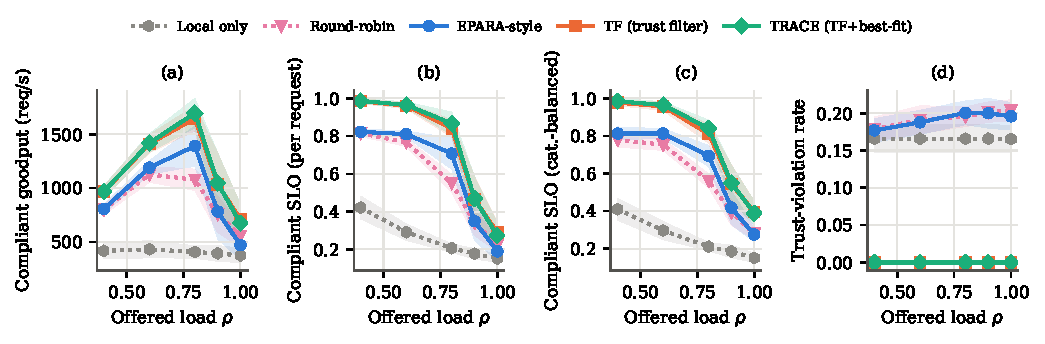
\includegraphics[width=\textwidth]{fig_load.pdf}
\caption{Routing under increasing offered load (30 servers, default sensitivity mix; mean and 95\% CI over 10 seeds). (a) Compliant goodput, (b) per-request and (c) category-balanced compliant SLO attainment, (d) fraction of requests served at a server that violates the trust constraint~\eqref{eq:elig}.}
\label{fig:load}
\end{figure*}

\begin{table*}[t]
\centering
\caption{Routers at offered load $\rho=0.8$ (mean $\pm$ 95\% CI, 10 seeds). SLO: raw SLO attainment; C-SLO: compliant SLO attainment, per request and category-balanced; Viol.: trust-violation rate; C-goodput: compliant goodput (req/s); Fwd.: forwards per request; $\mu$s: routing time per request in the Python prototype.}
\label{tab:main}
\footnotesize
\begin{tabular}{lccccccc}
\toprule
Policy & SLO & C-SLO & C-SLO$_{bal}$ & Viol. & C-goodput & Fwd. & $\mu$s \\
\midrule
Local only & 0.253$\pm$0.025 & 0.206$\pm$0.023 & 0.211$\pm$0.022 & 0.166$\pm$0.019 & 407$\pm$57 & 0.00$\pm$0.00 & 0.0$\pm$0.0 \\
Round-robin & 0.678$\pm$0.058 & 0.550$\pm$0.047 & 0.561$\pm$0.037 & 0.195$\pm$0.013 & 1078$\pm$99 & 1.25$\pm$0.08 & 1.5$\pm$0.1 \\
RR, shared pointer (ref.) & 0.720$\pm$0.043 & 0.574$\pm$0.033 & 0.582$\pm$0.023 & 0.203$\pm$0.016 & 1123$\pm$66 & 1.16$\pm$0.08 & 0.9$\pm$0.1 \\
EPARA-style & 0.883$\pm$0.110 & 0.708$\pm$0.082 & 0.694$\pm$0.056 & 0.200$\pm$0.016 & 1391$\pm$187 & 0.80$\pm$0.15 & 17.3$\pm$3.2 \\
TF (trust filter) & 0.841$\pm$0.046 & 0.841$\pm$0.046 & 0.812$\pm$0.049 & 0.000$\pm$0.000 & 1648$\pm$115 & 0.83$\pm$0.07 & 30.3$\pm$2.7 \\
\textbf{\sys{} (TF+best-fit)} & \textbf{0.867}$\pm$0.060 & \textbf{0.867}$\pm$0.060 & \textbf{0.841}$\pm$0.043 & \textbf{0.000}$\pm$0.000 & \textbf{1698}$\pm$135 & 0.78$\pm$0.10 & 31.9$\pm$3.6 \\
TF+EW (energy wt.) & 0.812$\pm$0.055 & 0.812$\pm$0.055 & 0.808$\pm$0.040 & 0.000$\pm$0.000 & 1590$\pm$108 & 0.91$\pm$0.11 & 36.7$\pm$4.3 \\
\bottomrule
\end{tabular}
\end{table*}

\subsection{Cost of compliance and the value of best-fit clearance}\label{sec:res-privacy}

Fig.~\ref{fig:privacy} varies the share of sensitive requests at $\rho=0.8$. The EPARA-style router's raw SLO attainment is unaffected by sensitivity (0.883 throughout) because it ignores it, but its violation rate grows linearly to 41\% when 80\% of requests are sensitive, so its compliant SLO falls from 0.883 to 0.523. Enforcing the constraint has a real cost: as sensitive traffic grows, the pool of eligible servers shrinks, and TF's raw (= compliant) SLO falls from 0.883 to 0.572. Even so, TF delivers more compliant service than the unconstrained router at every non-zero sensitive share, significantly so at 20--60\% ($+0.071$ to $+0.142$, $p\le0.037$).

Best-fit clearance targets exactly this regime. It improves compliant SLO over TF by $+0.027\pm0.015$ ($p=0.006$) at 40\% and $+0.051\pm0.024$ ($p=0.002$) at 60\% sensitive traffic. At 80\%, almost all traffic needs high clearance and there is little capacity left to reserve, so the gain shrinks ($+0.022$, $p=0.19$). With no sensitive traffic, best-fit only concentrates load on low-clearance servers and costs $-0.036$ (not significant, $p=0.084$). Table~\ref{tab:gamma} shows that at 60\% sensitive traffic any $\gamma\le0.3$ captures the benefit ($+0.051$ to $+0.055$ over $\gamma=1$, $p=0.002$). The gains in the category-balanced metric are smaller and not significant ($+0.015$ to $+0.025$), indicating that best-fit mainly helps the numerous short classification requests. In deployment, best-fit should therefore be enabled when a substantial share of traffic---roughly 30\% or more in our setting---is sensitive; the share is directly observable by each server.

\begin{figure}[t]
\centering
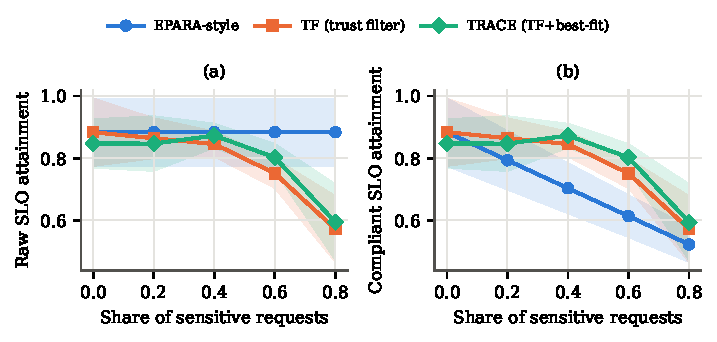
\includegraphics[width=\columnwidth]{fig_privacy.pdf}
\caption{Effect of the share of sensitive requests ($\rho=0.8$). (a) Raw SLO attainment ignores violations; (b) compliant SLO counts only lawful, timely requests. Bands are 95\% CIs across seeds; paired differences are reported in the text.}
\label{fig:privacy}
\end{figure}

\begin{table}[t]
\centering
\caption{Best-fit strength $\gamma$ with 60\% sensitive requests ($\rho=0.8$, 10 seeds). $\gamma=1$ is the plain trust filter.}
\label{tab:gamma}
\footnotesize
\begin{tabular}{ccc}
\toprule
$\gamma$ & C-SLO & C-SLO$_{bal}$\\
\midrule
1 (TF) & 0.751$\pm$0.049 & 0.761$\pm$0.051 \\
0.5 & 0.790$\pm$0.057 & 0.775$\pm$0.042 \\
0.3 (\sys) & 0.803$\pm$0.045 & 0.786$\pm$0.040 \\
0.1 & 0.806$\pm$0.055 & 0.789$\pm$0.045 \\
\bottomrule
\end{tabular}
\end{table}

\subsection{Energy-aware routing}\label{sec:res-energy}

Fig.~\ref{fig:energy} scales every server's energy cap from $1.0$ down to $0.35$ at $\rho=0.8$. The energy-weighted design does what it was meant to do locally: with unscaled caps it cuts the fraction of throttled requests from 8.4\% to 2.2\%. It does not, however, improve the quantity that matters.

\textbf{Soft throttling.} No energy-aware variant significantly outperforms TF at any energy level. TF+EW is never better and is significantly worse under scarce energy ($-0.100\pm0.052$ at cap scale 0.35, $p=0.002$). The barrier variant TF+EB loses $0.03$--$0.06$. Energy-as-capacity (TF+EC) is the best variant, within $\pm0.025$ of TF at every level (all $p\ge0.43$)---in other words, statistically indistinguishable from not modeling energy at all. Applying the energy weight without the trust filter (``EW only'') is the worst policy in every setting.

\textbf{Hard outage.} When drained servers go offline, every energy-aware variant is significantly worse than TF once energy is scarce (cap scale $\le0.7$, all $p=0.002$): by 0.18--0.23 for TF+EW, 0.10--0.14 for TF+EB and 0.23--0.28 for TF+EC. Energy awareness also \emph{lowers} server availability (at cap scale 0.5: 0.47 for TF vs.\ 0.40, 0.39 and 0.36) and raises drain events from 154 to 174--178 per minute.

\textbf{Ablation.} Table~\ref{tab:ablation} separates the energy weight $\beta$ from the retention threshold $\theta$ at cap scale 0.5. Compliant SLO decreases monotonically with $\beta$ under both energy models (outage: 0.568 at $\beta=0$, 0.438 at $\beta=0.5$, 0.334 at $\beta=1$, 0.317 at $\beta=2$). Retention alone ($\beta=0$, $\theta=0.25$) is neutral, slightly positive under soft throttling ($0.546$ vs.\ $0.518$) and slightly negative under outage ($0.556$ vs.\ $0.568$). The configuration of our original proposal ($\beta=1$, $\theta=0.25$) is among the worst.

\begin{figure*}[t]
\centering
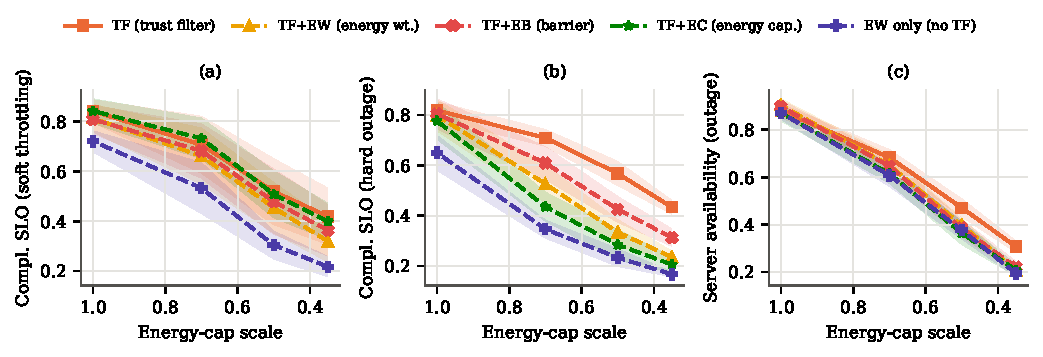
\includegraphics[width=\textwidth]{fig_energy.pdf}
\caption{Energy-aware variants as every server's energy cap is scaled down ($\rho=0.8$). (a) Compliant SLO under soft throttling; (b) compliant SLO and (c) mean server availability under the hard-outage model. The x-axis runs from abundant to scarce energy.}
\label{fig:energy}
\end{figure*}

\begin{table}[t]
\centering
\caption{Energy ablation for TF+EW at cap scale 0.5, $\rho=0.8$ (10 seeds): energy weight $\beta$ and retention threshold $\theta$. $\beta=\theta=0$ is TF.}
\label{tab:ablation}
\resizebox{\columnwidth}{!}{%
\begin{tabular}{cc|cc|ccc}
\toprule
 & & \multicolumn{2}{c|}{Soft throttling} & \multicolumn{3}{c}{Hard outage}\\
$\beta$ & $\theta$ & Compl. SLO & Throttled & Compl. SLO & Throttled & Avail. \\
\midrule
0 & 0 & 0.518$\pm$0.132 & 0.222$\pm$0.068 & 0.568$\pm$0.048 & 0.022$\pm$0.004 & 0.47$\pm$0.04 \\
0 & 0.25 & 0.546$\pm$0.136 & 0.220$\pm$0.069 & 0.556$\pm$0.034 & 0.018$\pm$0.005 & 0.47$\pm$0.04 \\
0.5 & 0 & 0.513$\pm$0.119 & 0.236$\pm$0.055 & 0.438$\pm$0.044 & 0.016$\pm$0.006 & 0.38$\pm$0.04 \\
1 & 0 & 0.469$\pm$0.111 & 0.209$\pm$0.052 & 0.334$\pm$0.043 & 0.011$\pm$0.005 & 0.39$\pm$0.05 \\
1 & 0.25 & 0.454$\pm$0.101 & 0.200$\pm$0.047 & 0.334$\pm$0.050 & 0.010$\pm$0.002 & 0.40$\pm$0.03 \\
1 & 0.4 & 0.463$\pm$0.109 & 0.206$\pm$0.051 & 0.346$\pm$0.048 & 0.009$\pm$0.002 & 0.39$\pm$0.04 \\
2 & 0.25 & 0.409$\pm$0.081 & 0.177$\pm$0.029 & 0.317$\pm$0.045 & 0.007$\pm$0.002 & 0.37$\pm$0.05 \\
\bottomrule
\end{tabular}}
\end{table}

\textbf{Is it stale information?} A natural explanation is herding: all servers see the same stale headroom values and pile onto the same ``energy-rich'' peers~\cite{mitzenmacher2000old}. If so, fresher state should shrink the penalty. Fig.~\ref{fig:estale} shows the opposite. Under hard outage, the penalty of TF+EW \emph{grows} as the sync period shrinks, from $-0.170$ at $H=2$\,s to $-0.388$ at $H=0.1$\,s (TF+EC: $-0.183$ to $-0.443$; all $p=0.002$), and availability falls with it. Stale information therefore does not cause the failure; the more accurately the router acts on energy headroom, the worse it does. We explain why in Section~\ref{sec:discussion}.

\begin{figure}[t]
\centering
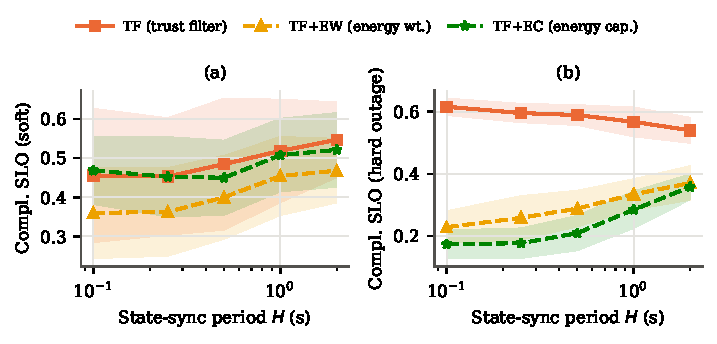
\includegraphics[width=\columnwidth]{fig_estale.pdf}
\caption{Energy-aware variants vs.\ the state-sync period $H$ (cap scale 0.5, $\rho=0.8$). Under hard outages (b), fresher state makes energy weighting worse, ruling out stale-information herding as the main cause.}
\label{fig:estale}
\end{figure}

\subsection{State staleness and saturation}\label{sec:res-stale}

Fig.~\ref{fig:stale} varies the sync period $H$ for the trust-oblivious routers and TF. At $\rho=0.8$, capacity-proportional routing is insensitive to staleness up to $H=1$\,s (EPARA-style 0.88--0.92, TF 0.84--0.86 raw SLO) and degrades at $H=2$\,s (TF 0.781).

At saturation ($\rho=1.0$) the effect reverses: fresher state \emph{hurts}. TF's raw SLO is 0.176 with $H=0.1$\,s but 0.289 with $H=1$\,s, and forwards per request fall from 1.08 to 0.80. The capacity view averages spare slots over a 0.5\,s horizon; when every server is saturated, a fresh view correctly reports almost no spare capacity, the offload weights collapse, and requests are served late locally. A stale view overstates spare capacity and keeps requests moving, so they find the short-lived free slots that 30\,ms classification jobs leave behind. Round-robin forwards regardless and therefore performs comparatively well at saturation (raw SLO 0.281). Even so, \sys{} retains a significant category-balanced advantage over round-robin at $\rho=1.0$ ($+0.109\pm0.051$, $p=0.004$), while the per-request difference is not significant ($+0.047$, $p=0.084$).

\textbf{The shared-pointer artifact.} A round-robin baseline whose pointer is shared by all servers---a natural implementation in a simulator---spreads load more evenly than any decentralized policy could, because it uses implicit global coordination. It overstates round-robin's compliant SLO at saturation by $+0.057\pm0.035$ ($p=0.014$); below saturation the difference is not significant. Our earlier experiments used the shared pointer and wrongly suggested that round-robin beats capacity-aware routing at saturation; we report the decentralized version throughout.

\begin{figure}[t]
\centering
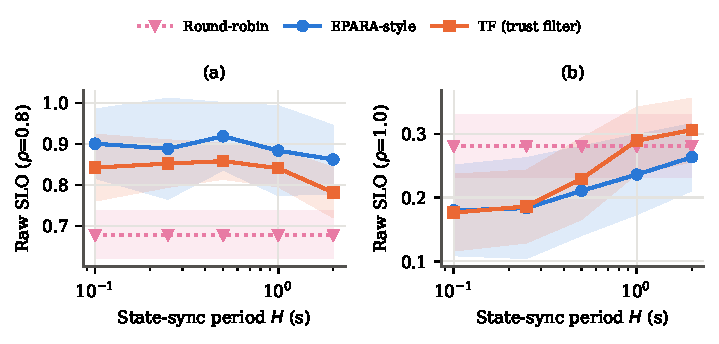
\includegraphics[width=\columnwidth]{fig_stale.pdf}
\caption{Sensitivity to the state-sync period $H$ at (a) $\rho=0.8$ and (b) $\rho=1.0$. At saturation, fresher state reduces forwarding and lowers SLO attainment of capacity-proportional routers.}
\label{fig:stale}
\end{figure}

\subsection{Scale and decision overhead}\label{sec:res-scale}

Fig.~\ref{fig:scale} varies the number of servers from 10 to 120 at $\rho=0.8$ (5 seeds). \sys{}'s compliant SLO attainment stays high and rises with scale (0.854 at $N=10$, 0.933 at $N=120$), because larger systems contain more eligible peers for every sensitivity level; TF follows the same trend at a lower level (0.823 to 0.883), and round-robin stays between 0.57 and 0.62. Routing time per request grows linearly with $N$, from 20\,$\mu$s at $N=10$ to 51\,$\mu$s at $N=120$, in an unoptimized Python implementation measured while seven simulations shared an 8-core Apple M3. This is three orders of magnitude below the 150\,ms SLO of the tightest service, and \sys{} adds only 2--3\,$\mu$s over TF. Since decisions use only local state, no communication is added on the request path.

\begin{figure}[t]
\centering
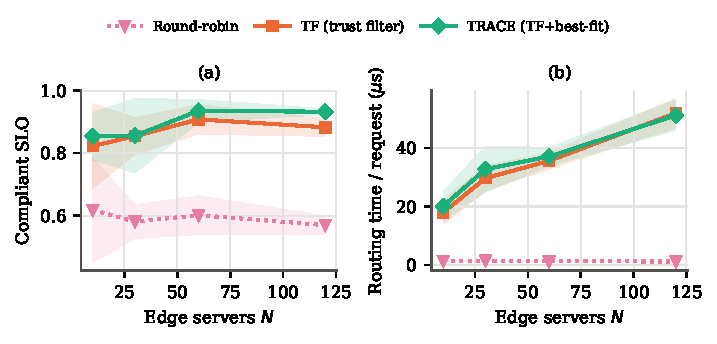
\includegraphics[width=\columnwidth]{fig_scale.pdf}
\caption{Scaling the number of edge servers ($\rho=0.8$, 5 seeds): (a) compliant SLO attainment, (b) routing time per request.}
\label{fig:scale}
\end{figure}

% =====================================================================
\section{Discussion}\label{sec:discussion}

\textbf{Why energy-aware routing fails.}
In our setting, energy is the binding resource, and every policy spends all of it: under the hard-outage model at cap scale 0.5, total power drawn is 10.0--10.6\,kW for all variants, and at most 0.1\% of the energy income is lost to full buffers. A router therefore cannot \emph{save} energy; it can only decide how much useful work each joule buys. TF spends 9.1\,J per successful request, TF+EW 16.7\,J and TF+EC 20.2\,J. Energy-aware routing loses for three related reasons.
(i) \emph{It is not work-conserving.} It declines compute that is free right now on servers with low headroom, even though serving a short request there would use energy those servers already hold.
(ii) \emph{It concentrates load.} Requests flow to whichever servers currently have the most energy, which drains them faster and synchronizes outages; availability falls (0.47 to 0.36--0.40) and drain events rise.
(iii) \emph{Weighting adds forwarding.} With TF+EW and TF+EB, forwards per request rise from 1.36 to 1.59 and 1.52, adding latency and missed SLOs. TF+EC forwards less (1.14) yet loses the most, consistent with (i) and (ii) dominating.
Because the first two effects grow with the accuracy of the headroom signal, fresher state makes them worse (Fig.~\ref{fig:estale}), which is the opposite of the herding signature. Our conclusion is that, at the per-request timescale, energy should enter routing only through \emph{local feasibility}---whether a server can run the request now without throttling---and not as a preference among peers. Energy-aware decisions belong at slower layers that can act on forecasts: service placement, admission control and DVFS.

\textbf{Averaged signals and fast jobs.}
The saturation result (Section~\ref{sec:res-stale}) and the energy result share a pattern: the router acts on a signal averaged over a horizon (0.5\,s of capacity, a 20\,s energy buffer) that is coarser than the jobs it routes (30\,ms classifications), and it acts on it too decisively. Sampling peers in proportion to the signal, rather than picking the best one, already softens this; a natural refinement is to keep a small exploration probability, or to use power-of-two choices~\cite{mitzenmacher2001two} over eligible peers, whenever the view says no peer has spare capacity. A preliminary test of uniform probing among eligible peers in that case did not help at saturation, so we leave the design of such a fallback to future work.

\textbf{Implications for EPARA-style systems.}
The trust filter is a small, local change to EPARA's handler: it adds a per-peer eligibility test, keeps decisions in tens of microseconds and needs only static clearance and domain labels in the synchronized state. Given that trust-oblivious handlers serve about one in five requests unlawfully under our assumptions, we argue that compliant goodput, not raw goodput, should be the headline metric for edge inference systems that handle regulated data.

\textbf{Threats to validity and limitations.}
\emph{Simulation only.} All results come from an event-driven simulator. Service times, slot power, clearance and domain distributions, energy caps and the network model are assumptions modeled on EPARA's testbed scale, not measurements; absolute values should not be compared with EPARA's results~\cite{epara2025}. The qualitative conclusions---violation rates set by the fraction of ineligible servers, the cost of compliance growing with sensitive share, and energy-aware routing being non-work-conserving---depend on the structure of the problem rather than on specific constants, but we have not verified them on hardware.
\emph{Workload.} Arrivals are synthetic (Poisson with hot spots and bursts), not the Azure function and LLM traces used by EPARA~\cite{shahrad2020serverless,epara2025}.
\emph{Fixed layers.} Service placement and operator selection are fixed and identical across policies; we do not evaluate trust-aware placement, which could reduce the cost of compliance further.
\emph{Trust model.} Clearance and domains are static labels with a single eligibility rule~\eqref{eq:elig}; real policies (consent, purpose limitation, cross-border transfer rules) are richer.
\emph{Energy model.} Energy is a leaky bucket with fixed per-slot power; DVFS, idle power and cooling are not modeled.
\emph{Statistics and tuning.} Each configuration was run for 30\,s with 10 seeds (5 in the scale study); confidence intervals across seeds are wide because topologies differ, so we base claims on paired tests. $\gamma$ was selected at a single sensitivity level.
\emph{Timing.} Routing times are from an unoptimized Python prototype on a shared machine and are indicative only.

% =====================================================================
\section{Conclusion}\label{sec:conclusion}

Decentralized, capacity-proportional request routing is an effective way to pool the scattered capacity of edge servers for AI inference, but routers designed this way treat every server as a lawful destination. We formalized trust-constrained routing for EPARA-style categorized inference, defined compliant goodput, and proposed \sys{}, which adds a hard trust filter and a best-fit clearance preference to capacity-proportional offloading at a cost of tens of microseconds per decision. In simulation, trust-oblivious routers serve roughly one in five requests outside its trust boundary at every load. \sys{} eliminates these violations and raises compliant goodput over an EPARA-style router; best-fit clearance helps further when much of the traffic is sensitive. Energy-headroom weighting, which we had expected to help on power-capped and battery-backed sites, did not improve compliant SLO attainment in any variant we tried and hurt substantially when drained servers go offline.

The next steps are to replace the assumed service and power profiles with measurements on edge hardware, to drive the simulator with production traces, to co-design trust-aware service placement with the router, to adapt the best-fit strength online, and to revisit energy awareness at the placement and admission-control layers, where it can act on forecasts rather than on a stale per-request signal.

% ---- References (embedded; generated from refs.bib with IEEEtran.bst) ----
% To manage references with BibTeX instead, replace this block with:
%   \bibliographystyle{IEEEtran}
%   \bibliography{refs}
% Generated by IEEEtran.bst, version: 1.14 (2015/08/26)
\begin{thebibliography}{10}
\providecommand{\url}[1]{#1}
\csname url@samestyle\endcsname
\providecommand{\newblock}{\relax}
\providecommand{\bibinfo}[2]{#2}
\providecommand{\BIBentrySTDinterwordspacing}{\spaceskip=0pt\relax}
\providecommand{\BIBentryALTinterwordstretchfactor}{4}
\providecommand{\BIBentryALTinterwordspacing}{\spaceskip=\fontdimen2\font plus
\BIBentryALTinterwordstretchfactor\fontdimen3\font minus
  \fontdimen4\font\relax}
\providecommand{\BIBforeignlanguage}[2]{{%
\expandafter\ifx\csname l@#1\endcsname\relax
\typeout{** WARNING: IEEEtran.bst: No hyphenation pattern has been}%
\typeout{** loaded for the language `#1'. Using the pattern for}%
\typeout{** the default language instead.}%
\else
\language=\csname l@#1\endcsname
\fi
#2}}
\providecommand{\BIBdecl}{\relax}
\BIBdecl

\bibitem{liu2025eccc}
J.~Liu, Y.~Du, K.~Yang, Y.~Wang, X.~Hu, Z.~Wang, Y.~Liu, P.~Sun, A.~Boukerche,
  and V.~C.~M. Leung, ``Edge-cloud collaborative computing on distributed
  intelligence and model optimization: A survey,'' \emph{arXiv preprint
  arXiv:2505.01821}, 2025.

\bibitem{epara2025}
Y.~Wang, Y.~Cui, T.~Shi, D.~Li, W.~Li, L.~Suo, T.~Wang, and X.~Xie, ``{EPARA}:
  Parallelizing categorized {AI} inference in edge clouds,'' \emph{arXiv
  preprint arXiv:2511.00603}, 2025.

\bibitem{interedge}
L.~Brown, E.~Marx, D.~Bali, E.~Amaro, D.~Sur \emph{et~al.}, ``An architecture
  for edge networking services,'' in \emph{Proc. ACM SIGCOMM}, 2024, pp.
  645--660.

\bibitem{galaxy}
S.~Ye, J.~Du, L.~Zeng, W.~Ou, X.~Chu \emph{et~al.}, ``Galaxy: A
  resource-efficient collaborative edge {AI} system for in-situ transformer
  inference,'' in \emph{Proc. IEEE INFOCOM}, 2024, pp. 1001--1010.

\bibitem{servp}
V.~Farhadi, F.~Mehmeti, T.~He, T.~F. La~Porta, H.~Khamfroush \emph{et~al.},
  ``Service placement and request scheduling for data-intensive applications in
  edge clouds,'' \emph{IEEE/ACM Trans. Netw.}, vol.~29, no.~2, pp. 779--792,
  2021.

\bibitem{alpaserve}
Z.~Li, L.~Zheng, Y.~Zhong, V.~Liu, Y.~Sheng \emph{et~al.}, ``{AlpaServe}:
  Statistical multiplexing with model parallelism for deep learning serving,''
  in \emph{Proc. USENIX OSDI}, 2023, pp. 663--679.

\bibitem{usher}
S.~S. Shubha, H.~Shen, and A.~Iyer, ``{USHER}: Holistic interference avoidance
  for resource optimized {ML} inference,'' in \emph{Proc. USENIX OSDI}, 2024,
  pp. 947--964.

\bibitem{gdpr}
{European Parliament and Council}, ``Regulation ({EU}) 2016/679 ({General Data
  Protection Regulation}),'' Official Journal of the European Union, L 119,
  2016.

\bibitem{mao2016harvest}
Y.~Mao, J.~Zhang, and K.~B. Letaief, ``Dynamic computation offloading for
  mobile-edge computing with energy harvesting devices,'' \emph{IEEE J. Sel.
  Areas Commun.}, vol.~34, no.~12, pp. 3590--3605, 2016.

\bibitem{min2019privacy}
M.~Min, X.~Wan, L.~Xiao, Y.~Chen, M.~Xia, D.~Wu, and H.~Dai, ``Learning-based
  privacy-aware offloading for healthcare {IoT} with energy harvesting,''
  \emph{IEEE Internet Things J.}, vol.~6, no.~3, pp. 4307--4316, 2019.

\bibitem{fisher1978submodular}
M.~L. Fisher, G.~L. Nemhauser, and L.~A. Wolsey, ``An analysis of
  approximations for maximizing submodular set functions---{II},''
  \emph{Mathematical Programming Study}, vol.~8, pp. 73--87, 1978.

\bibitem{nexus}
H.~Shen, L.~Chen, Y.~Jin, L.~Zhao, B.~Kong \emph{et~al.}, ``Nexus: A {GPU}
  cluster engine for accelerating {DNN}-based video analysis,'' in \emph{Proc.
  ACM SOSP}, 2019, pp. 322--337.

\bibitem{shepherd}
H.~Zhang, Y.~Tang, A.~Khandelwal, and I.~Stoica, ``{SHEPHERD}: Serving {DNNs}
  in the wild,'' in \emph{Proc. USENIX NSDI}, 2023, pp. 787--808.

\bibitem{clockwork}
A.~Gujarati, R.~Karimi, S.~Alzayat, W.~Hao, A.~Kaufmann, Y.~Vigfusson, and
  J.~Mace, ``Serving {DNNs} like clockwork: Performance predictability from the
  bottom up,'' in \emph{Proc. USENIX OSDI}, 2020, pp. 443--462.

\bibitem{infaas}
F.~Romero, Q.~Li, N.~J. Yadwadkar, and C.~Kozyrakis, ``{INFaaS}: Automated
  model-less inference serving,'' in \emph{Proc. USENIX ATC}, 2021, pp.
  397--411.

\bibitem{neurosurgeon}
Y.~Kang, J.~Hauswald, C.~Gao, A.~Rovinski, T.~Mudge, J.~Mars, and L.~Tang,
  ``Neurosurgeon: Collaborative intelligence between the cloud and mobile
  edge,'' in \emph{Proc. ACM ASPLOS}, 2017, pp. 615--629.

\bibitem{edgeshard}
M.~Zhang, J.~Cao, X.~Shen, and Z.~Cui, ``{EdgeShard}: Efficient {LLM} inference
  via collaborative edge computing,'' \emph{arXiv preprint arXiv:2405.14371},
  2024.

\bibitem{mcmahan2017fl}
B.~McMahan, E.~Moore, D.~Ramage, S.~Hampson, and B.~{Ag{\"u}era y Arcas},
  ``Communication-efficient learning of deep networks from decentralized
  data,'' in \emph{Proc. AISTATS}, 2017, pp. 1273--1282.

\bibitem{ecoserve}
Y.~Li, Z.~Hu, E.~Choukse, R.~Fonseca, G.~E. Suh, and U.~Gupta, ``{EcoServe}:
  Designing carbon-aware {AI} inference systems,'' \emph{arXiv preprint
  arXiv:2502.05043}, 2025.

\bibitem{mitzenmacher2000old}
M.~Mitzenmacher, ``How useful is old information?'' \emph{IEEE Trans. Parallel
  Distrib. Syst.}, vol.~11, no.~1, pp. 6--20, 2000.

\bibitem{mitzenmacher2001two}
------, ``The power of two choices in randomized load balancing,'' \emph{IEEE
  Trans. Parallel Distrib. Syst.}, vol.~12, no.~10, pp. 1094--1104, 2001.

\bibitem{shahrad2020serverless}
M.~Shahrad, R.~Fonseca, {\'I}.~Goiri, G.~Chaudhry, P.~Batum, J.~Cooke,
  E.~Laureano, C.~Tresness, M.~Russinovich, and R.~Bianchini, ``Serverless in
  the wild: Characterizing and optimizing the serverless workload at a large
  cloud provider,'' in \emph{Proc. USENIX ATC}, 2020, pp. 205--218.

\end{thebibliography}

\end{document}
